%
%\subsection{Experimental Procedure}
%\paragraph{}
%Each experiment commenced with extensive sample preparation: in which the Westerly granite was cut and notched, sealed in a latex jacket, and then placed inside the pressure vessel (see Section \ref{sec:experimnt_setup} for details). After sealing the pressure vessel and loading the sample, inlet and outlet flow were pressurized to 4 MPa and 2MPa, respectively. At this stage there was no flow because Westerly granite matrix permeability is very low ($< 10^{-20}\ m^2$ ) and the confining fluid pressure (around the jacketed sample) is much larger than the pore pressure, preventing flow of water around the sample.
%A shear load was then applied with the vertical piston in displacement mode at a constant 10 $\mu m/s$, fracturing in-situ after reaching a critical stress of $ \approx $60 MPa, and then locked the vertical piston. During fracture fluid flow and acoustic emissions were measured, but these results are not included in this paper. Next, the dynamic stressing protocol was implemented in which the normal stress and pore pressure were modulated. Normal stress oscillations were applied by oscillating the horizontal piston of the load frame at prescribed amplitudes (0.2 to 3 MPa) and frequencies (0.1, 1, 10, 40 Hz). Pore pressure oscillations were achieved by oscillating $P_{PA}$ while holding $P_{PB}$ constant at amplitudes of 0.2 to 3 MPa and frequencies of 0.1, 1, 10 Hz. Multiple sets of normal stress and pore pressure oscillations of varying amplitudes and frequencies were applied to investigate: (1) repeatability and direct comparison between the two modulated stresses and (2) amplitude and frequency dependencies of the measured response. Post-fracture dynamic stressing is plotted in Figure \ref{fig:exp_seq}d (highlighted in yellow) and shows the normal stress (red) and pore pressure (blue) oscillations; note that line thickness correlates with oscillation frequency. 
%To investigate the effect of fracture aperture on elastic nonlinearity and permeability, the sample was sheared in two 4 mm, (held at $ \sigma_{NS} $ = 20 MPa) stages. After each shearing stage the oscillation protocol was applied to the sample. Initially,the in-situ fracture was quite rough, but the effect of shear reduces and changes this roughness; the old contacts were broken and new contacts formed, changing the extent to which the two halves of the fracture were mated. This allows for investigation of how fracture aperture is related to the elasto-dyamic and hydromechanical properties. 
%
%\newpage
%
%
%\begin{figure*}[ht]
%	\centering
%	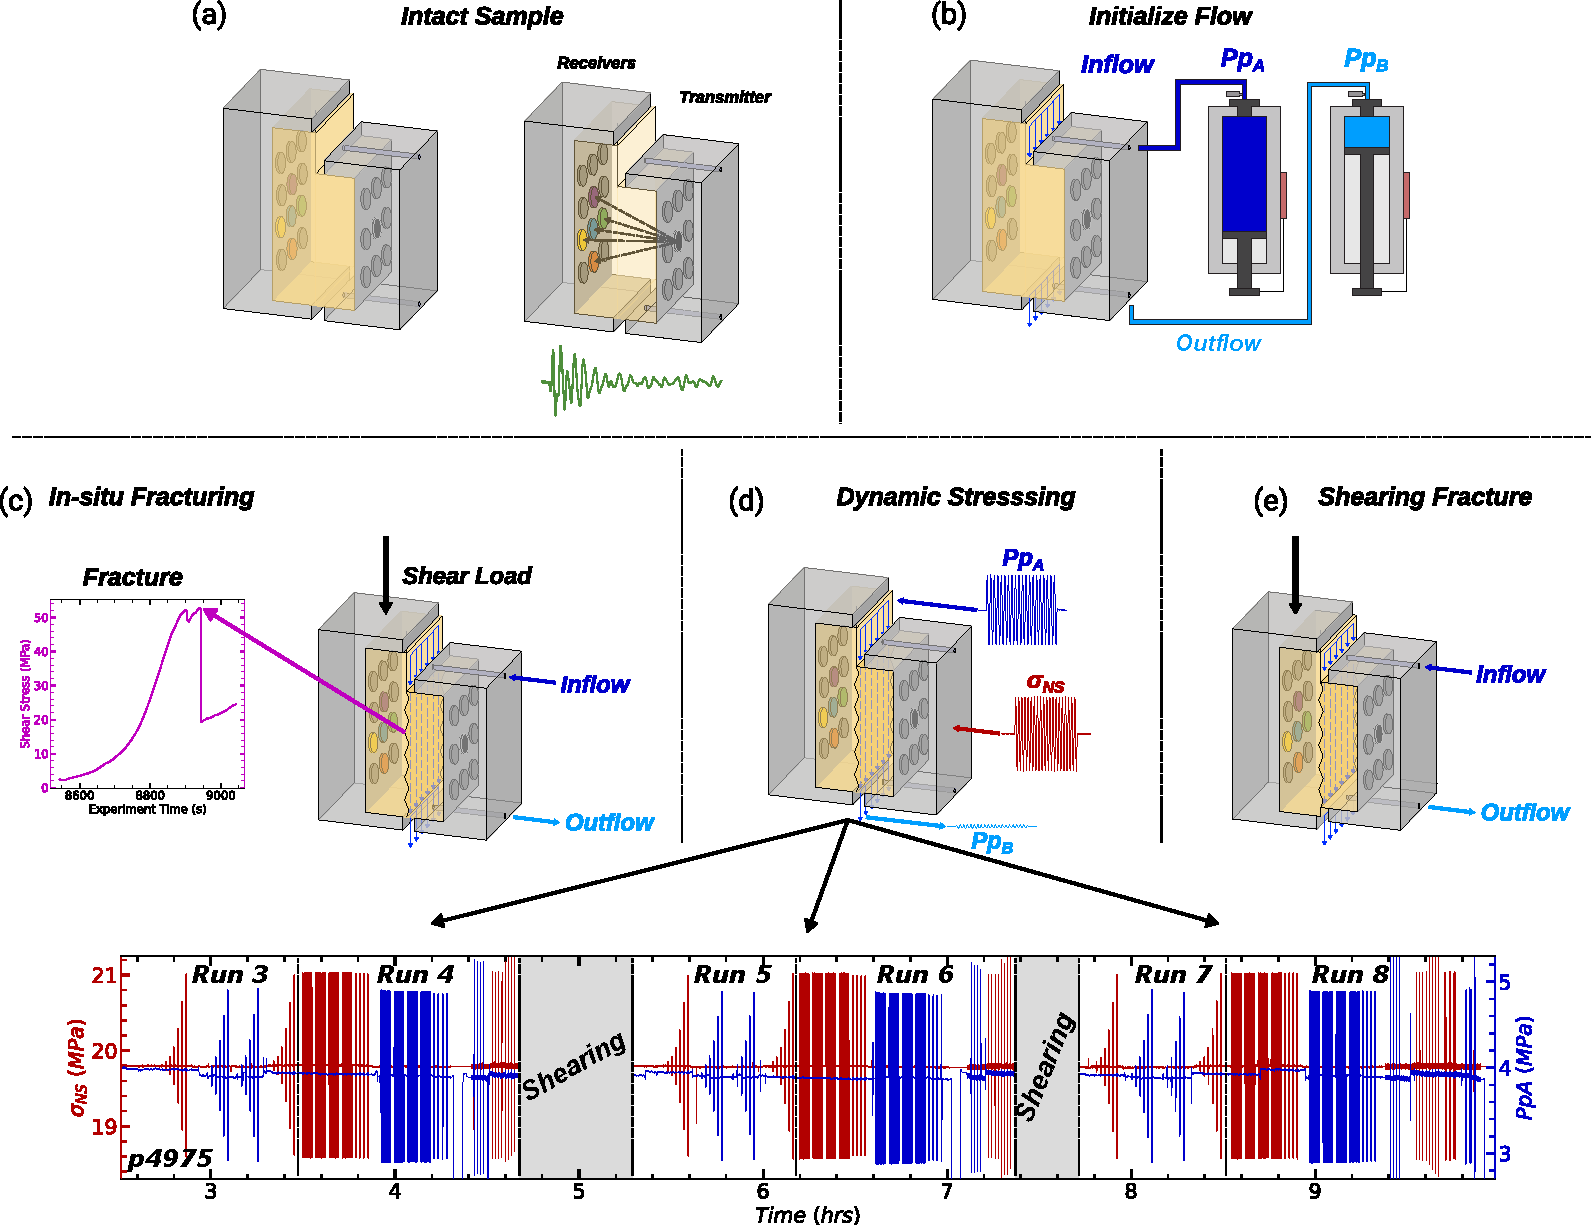
\includegraphics[width=0.99\columnwidth]{exp_sequence_v2}
%	\caption[]{(a) Intact Westerly granite sample cartoon, showing dimensions and approximate transmitter - receiver ray paths. 
%	(b) Next, we applied a pore pressure differential: inlet ($P_{PA}$ = 4 MPa) and outlet ($P_{PB}$ = 2 MPa). 
%	(c) The shear stress was loaded at a constant rate of 10 $\mu m/s$ until reaching the critical shear stress at $ \approx $60 MPa. 
%	(d) Cartoon showing the oscillation protocol applied to the freshly fractured sample. Multiple sets of $P_{P}$ and $ \sigma_{NS} $ oscillations of varying amplitude (up to about $ \pm $ 1 MPa) and frequency (0.1, 1, 10 and 40 Hz) were applied. 
%	(e) The sample was sheared in two additional increments of 4mm, each followed by the dynamic stressing protocol.}
%	\label{fig:exp_seq}
%\end{figure*}
%
%
%\newpage